% Copyright (c) 2008-2009 solvethis
% Copyright (c) 2010-2011 Casper Ti. Vector
% Public domain.

\chapter{机器学习类震级预估算法}

\indent 考虑到特征频率和特征幅值两类算法的局限性,本文选取了机器学习中神经网络类算法进行对传统方法进行改进。神经元是构成神经网络最基础的单元,它的结构可抽象成如下图1所示的简单数学模型 (McCulloch and Pitts, 1943),即“M-P神经元模型”。在这个模型中,一个神经元接收到来自n个其他神经元传递过来的输入信号$\mathrm{X}_{\mathrm{i}}$,这些输入信号通过带权重$\mathrm{w}_{\mathrm{i}}$的连接方式进行传递,并将神经元接收到的总输入值$\sum_{i=1}^{n} W_{i} x_{i}$将与神经元的阀值θ进行比较,然后通过“激活函数”处理以产生神经元的输出,这样就完成一个神经元的运算过程。把许多个这样的神经元按一定的层次结构连接起来,就得到各种结构的神经网络。
    
\begin{figure}[!h]
\centerin
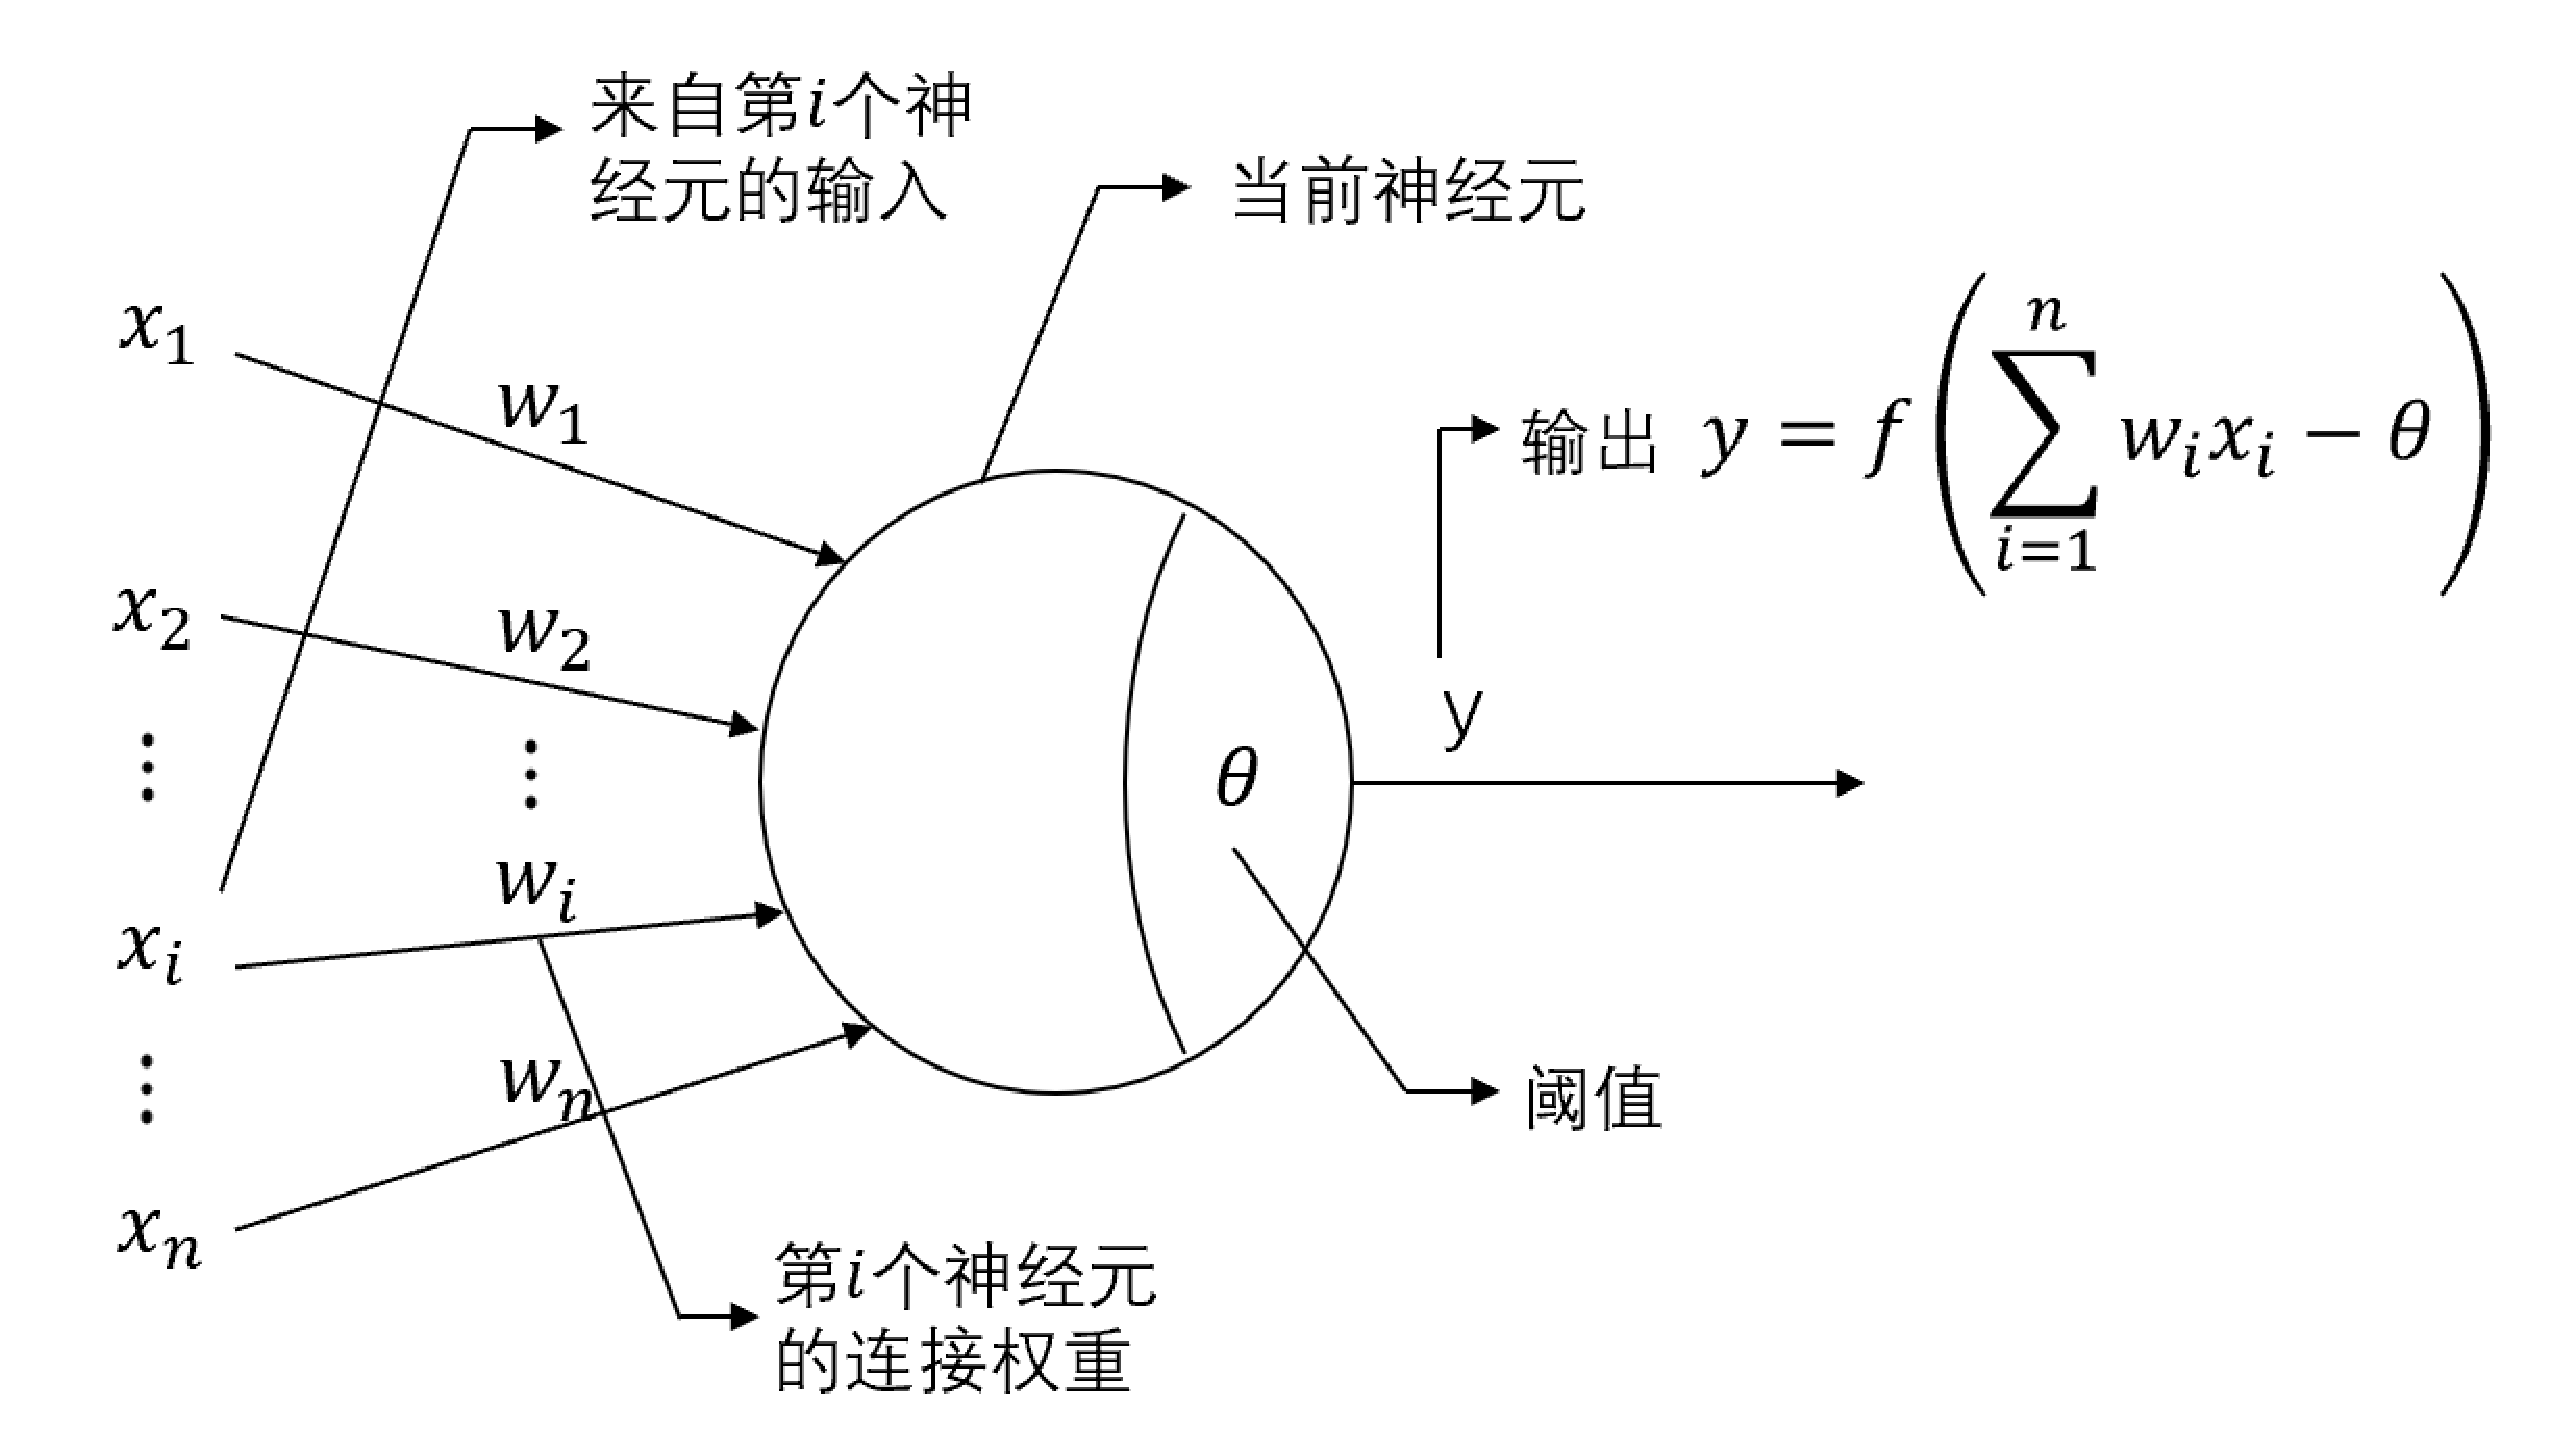
\includegraphics[width=0.99\linewidth]{img/mp.eps}
\caption{ 平面断层破裂过程} \label{fig:rupture-process}
\end{figure}

\indent 我们按照不同训练思路设计出两种神经网络模型用以预估震级。损失函数是机器学习模型效果的评判标准,通过调整模型参数来最小化损失函数以达到优化模型性能的目的。本研究的两种模型的训练目标都按(9)式设置,使用平方误差作为损失函数L。将模型设置为回归问题进行训练,通过(8)式使用BP算法采用梯度下降的方式最小化损失函数以得到优化的神经网络权值$\theta^{*}$(Werbos, 1974; Rumelhart et al., 1986a,b),其中$\mathrm{W}_{\mathrm{i}}$代表第i个隐藏层。同时如下(9)式加入网络权值的$\mathrm{L}_{1}$、$\mathrm{L}_{2}$范数的进行正则约束以防止过拟合。

\begin{equation}
\theta^{*}=\arg \min \frac{1}{N} \sum_{i=1}^{N} L\left(y_{i}, f\left(x_{i} ; \theta_{i}\right)\right)+\sum_{q=1}^{z} \Phi\left(W_{q}\right)
\end{equation}
\begin{equation}
\left\{\begin{array}{c}{L\left(y_{i}, f\left(x_{i}\right)\right)=\left|y_{i}-f\left(x_{i}\right)\right|^{2}} \\ {\Phi\left(W_{q}\right)=\lambda_{1}\left|W_{q}\right|+\lambda_{2} W_{q}^{2}}\end{array}\right.
\end{equation}

其中arg⁡min算符定义为$\theta^{*}=\arg \min f(\theta)$下,使$f(\theta)$达到最小值的$\theta$值,N为采用mini-batch方式每次训练抽样数量的大小,z代表隐藏的层数。

\indent NN模型结构如图2所示,整体框架为全连接神经网络。隐藏层间连接方式为下(10)和(11)式,
\begin{equation}
\mathrm{Z}_{\mathrm{c}}^{i}=\sigma\left(b_{c}^{i}+\sum_{c^{\prime}=1}^{c_{i}} Z_{C^{\prime}}^{i-1} \cdot W_{C C^{\prime}}^{i}\right)
\end{equation}
\begin{equation}
\sigma(x)=\max (0, x)
\end{equation}



其中下角标C,$C^{\prime}$代表了输出层和输入层,上角标i代表第i个隐藏层。激活函数使用(11)式中所示的以0为分界的分段函数ReLU(Alex et al., 2012)。当此激活函数接收到前一隐层小于0的输入时输出0,而当接收到大于0的隐藏层输入时不做处理直接作为输出。NN模型以特征频率类方法的思想为基础,但区别于$\tau_{\mathrm{C}}$方法只使用垂直分量的信息,此NN神经网络的使用台站记录的全三分量信息,以期望得到不同分量联合与破裂规模的关系。将3s时窗内的三分量频谱信息并列为一维张量(tensor)作为模型输入,预估的震级结果作为模型输出。整个模型共有7层神经网络,除去首尾的输入、输出层外共设置5个隐藏层。根据Hinton(2012a,2012b)和Alex(2012),我们在第1和第3隐层后连接Dropout层以防止过拟合,同时加快有效训练速率。

    
\begin{figure}[!h]
  \centerin
  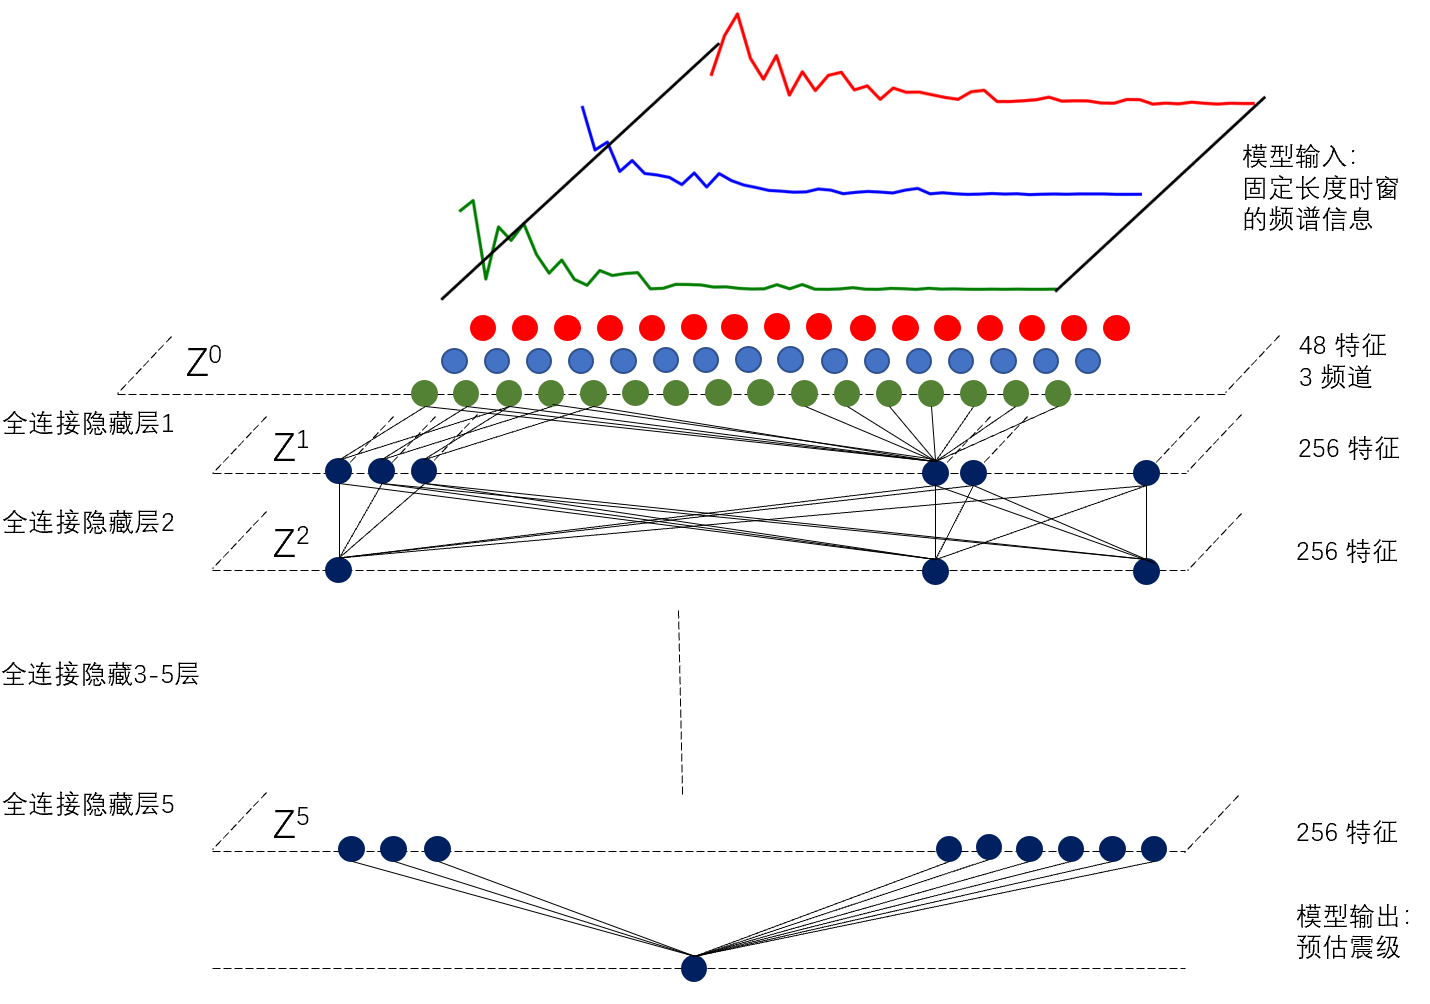
\includegraphics[width=0.99\linewidth]{img/NN.png}
    \caption{ 平面断层破裂过程} \label{fig:rupture-process}
 \end{figure}

\begin{figure}[!h]
  \centerin
  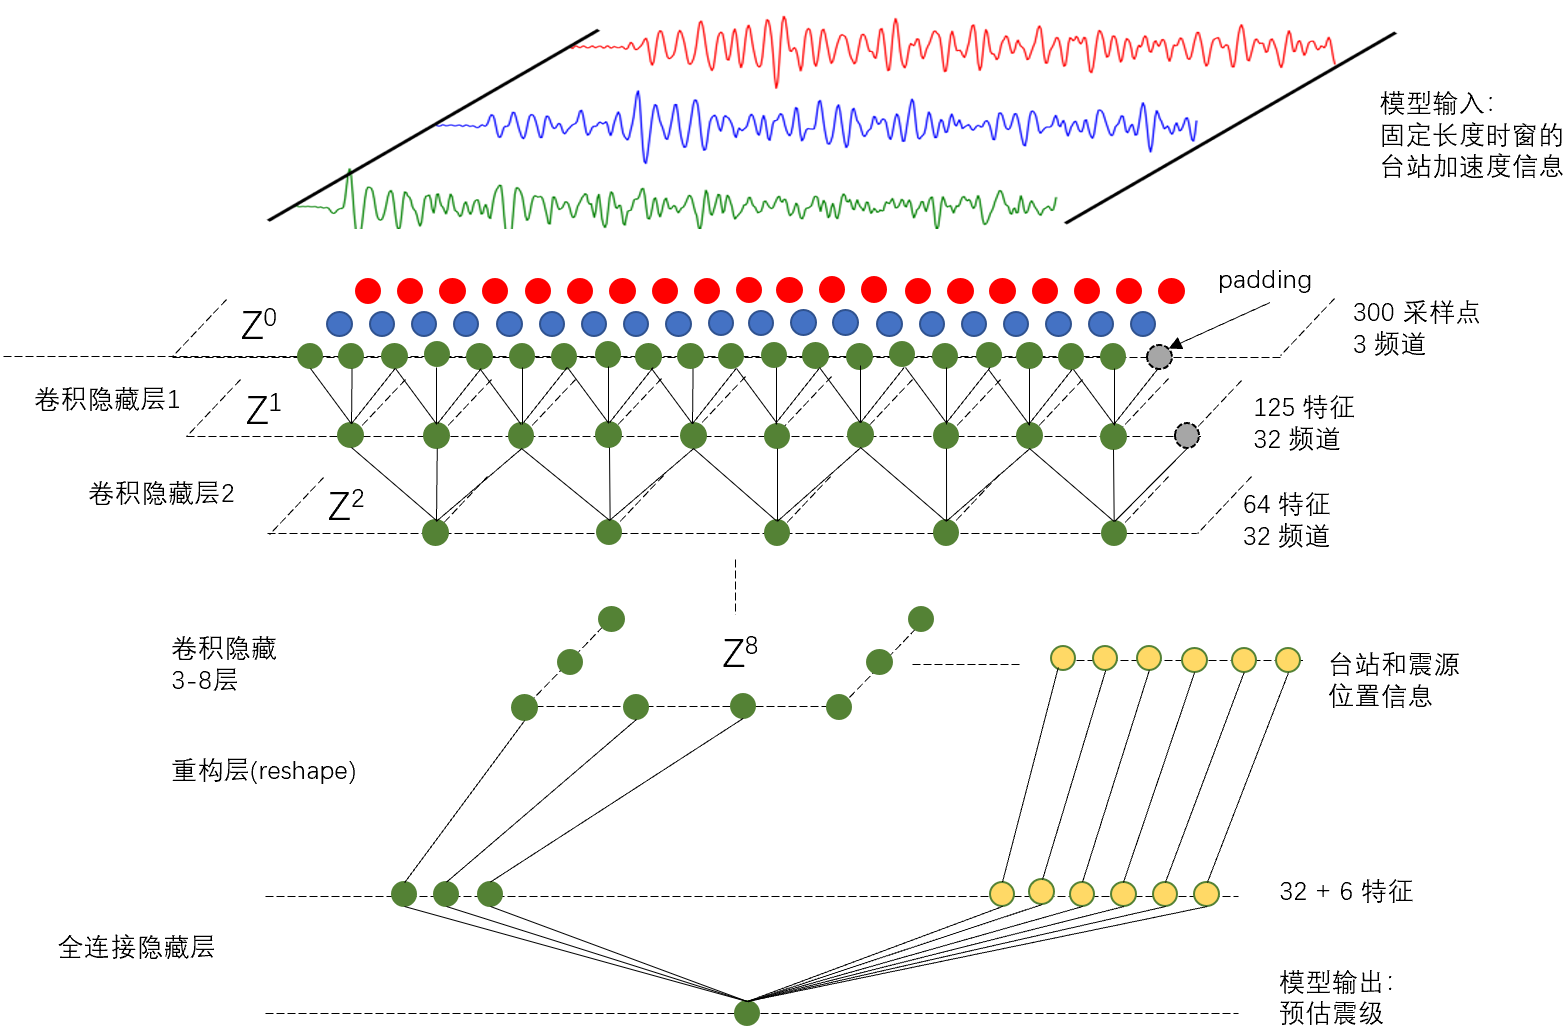
\includegraphics[width=0.99\linewidth]{img/CNN.png}
    \caption{ 平面断层破裂过程} \label{fig:rupture-process}
 \end{figure} 


